\documentclass[10pt]{article}

\usepackage[pdftex]{graphicx}
\usepackage{amsmath}
\usepackage{amsthm}
\theoremstyle{theorem}
\newtheorem{theorem}{Rule} % define rules in theorem style
\usepackage{mathtools}
\usepackage{pythonhighlight}
\usepackage[backend=bibtex]{biblatex}
\addbibresource{zigzag.bib}


%-------------------------------------------------------------------------------

\begin{document}

\title{\LARGE Properties of the Zigzag Space Filling Curve}
\author{piers.barber@logicmonkey.co.uk}

\maketitle

\begin{abstract}
  Interesting properties of the Zigzag space filling curve are presented.
  Methods for the calculation of positions on the curve are shown, specifically
  a method to convert a Cartesian coordinate to a parametric distance along the
  curve and, the inverse of this operation.
\end{abstract}

%-------------------------------------------------------------------------------

\section{Introduction}

Searches for literature on the zigzag space filling curve don't yield too
many results. It does not seem to have been studied to much depth in many
places, presumably because there are other curves that are recursive and
with simpler parametric and coordinate representations: for example, the
Hilbert-Peano \cite{hilbert} and Morton Order (Z) \cite{zfill}  curves. The
zigzag may be of limited use, but it does fill square regions of arbitrary
width and height (non powers of two) without loss of generality.

\begin{figure}[h]
  \centering
  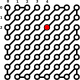
\includegraphics[width=2.5in]{zz_example}
  \caption{Example $\mathbf{8\times8}$ zigzag with highlighted node S=23
  $\Leftrightarrow$ XY=(4,2)}
  \label{fig:example}
\end{figure}

The zigzag space filling curve of Fig.~\ref{fig:example} is mainly used in MPEG
\cite{mpeg} and JPEG \cite{jpeg} encode/decode.  Implementations generally use
a 64 entry look up table to convert between a linear address and an
$\mathbf{8\times8}$ array entry.  It's a simple solution, but it hides
interesting attributes of the curve that can be calculated in real time rather
than looked up.

This article will show how we can:
\begin{itemize}
  \item convert parametric distance S along the curve to Cartesian coordinates,
  \item convert Cartesian coordinates to parametric distance S,
  \item constrain the curve to a square region without the need for bounding
    box checks,
  \item implement the calculations in hardware (RTL).
    \footnote{Python that refactors readily to an HDL for RTL synthesis.
    Pytherilog\texttrademark ?}
\end{itemize}

%-------------------------------------------------------------------------------

\section{Properties}

\subsection{General}
Fig.~\ref{fig:infinite} shows points on the curve over an unbounded region.
Note the following properties:

\begin{theorem} \label{thm:diagconstant}
  The sum of the XY coordinates is constant and unique along each diagonal
\end{theorem}
\begin{theorem} \label{thm:diagtrinum}
  Each diagonal starts with a triangular number.
  \footnote{The $\mathbf{n}$th triangular number $\mathbf{T_n}$ is the sum of all
    natural numbers from $\mathbf{1}$ to $\mathbf{n}$}
  $\mathbf{T_n}$
\end{theorem}
\begin{theorem} \label{thm:diagevenodd}
  The sum of the XY coordinates alternates even/odd from one diagonal to the
  next. Adjacent diagonals run in opposite directions.
\end{theorem}
\begin{theorem} \label{thm:diagtriroot}
  The sum of the XY coordinates along a diagonal is the triangular root
  \footnote{For a number $\mathbf{k}$ on the diagonal, the triangular root of
    $\mathbf{k}$ is the natural number $\mathbf{n}$ that has the highest
    triangular number $\mathbf{T_n \leq k}$.}
  of all numbers on that diagonal.
\end{theorem}

\begin{figure}[h]
  \centering
  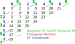
\includegraphics[width=3.45in]{zz_infinite}
  \caption{Unbounded zigzag}
  \label{fig:infinite}
\end{figure}

These rules allow us to navigate within the space using both the parametric
distance along the curve and the XY position.

\subsection{Bounded Regions}

Fig.~\ref{fig:bounded} is an example of a zigzag curve bounded to
$\mathbf{5\times5}$ points.  Left unbounded, the curve strays outside of the
required region for points to the right of the principal (longest) diagonal.
Other points stray into the bounded region. We can correct this behaviour by
noting that there is symmetry around the principal diagonal and reflecting each
point to its right onto a corresponding correctly numbered point on its left.

\begin{theorem} \label{thm:principaldiag}
  For an $\mathbf{N \times N}$ bound, the principal diagonal has an XY
  coordinate sum (triangular root) of $\mathbf{x+y=N-1}$.
\end{theorem}
\begin{theorem} \label{thm:curvemidpoint}
  Points at a distance greater than half way along the curve are considered to
  be to the right of the principal diagonal (and have a reflectively translated
  counter position to the left of the principal diagonal).
\end{theorem}
\begin{theorem} \label{thm:boundednontri}
  Bounded diagonals to the right of the principal diagonal do not in general
  start on a triangular number.
\end{theorem}

\begin{figure}[h]
  \centering
  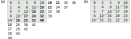
\includegraphics[width=3.45in]{zz_bounded}
  \caption{Bounding: (a) Unconstrained behaviour, errors in bold. (b)
  Constrained behaviour, reflection around principal diagonal}
  \label{fig:bounded}
\end{figure}

%-------------------------------------------------------------------------------

\section{Mapping XY to distance S}

We assume a bounding box of $\mathbf{N \times N}$ and Cartesian coordinates
$\mathbf{(x, y)}$ such that
\[
  \mathbf{0 \leq x \leq N-1, 0 \leq y \leq N-1}
\]
To find the distance $\mathbf{S}$ along the curve for some point $\mathbf{P}$
at position $\mathbf{(x_p,y_p)}$, the approach is:
\begin{enumerate}
  \item Find the triangular root of the diagonal that $\mathbf{P}$ lies on
    (Rule~\ref{thm:diagconstant}):
    \[\mathbf{n=x_p+y_p}\]
  \item Translate $\mathbf{P}$ to $\mathbf{(x_t,y_t)}$
    (Rule~\ref{thm:principaldiag}):
    \begin{align}
      \mathbf{(x_t,y_t) =}
      \begin{cases*}
        \mathbf{(x_p, y_p)}, & if $\mathbf{n \leq N-1}$ no change \\
        \mathbf{(N-1-x_p, N-1-y_p)}, & otherwise right of principal diagonal. \\
      \end{cases*} \notag
    \end{align}
  \item Calculate the diagonal's triangular number starting position
    (Rule~\ref{thm:diagtrinum}):
    \begin{equation}\label{eqn:triangular}
      \mathbf{T_n=\frac{n(n+1)}{2}}
    \end{equation}
  \item Offset from the diagonal's start either up and to the right with $\mathbf{x_t}$
    or down and to the left with $\mathbf{y_t}$ (Rule~\ref{thm:diagevenodd}):
    \begin{align}
      \mathbf{U =}
      \begin{cases*}
        \mathbf{T_n + x_t}, & if $\mathbf{n}$ is odd \\
        \mathbf{T_n + y_t}, & if $\mathbf{n}$ is even. \\
      \end{cases*} \notag
    \end{align}
  \item Translate back if originally right of the principal diagonal
    (Rule~\ref{thm:principaldiag}):

    \begin{align}
      \mathbf{S =}
      \begin{cases*}
        \mathbf{U}, & if $\mathbf{n \leq N-1}$ no change \\
        \mathbf{N^2-1-U}, & otherwise offset back from bottom right. \\
      \end{cases*} \notag
    \end{align}

\end{enumerate}

%-------------------------------------------------------------------------------

\section{Mapping distance S to XY}

We assume a bounding box of $\mathbf{N \times N}$ and Cartesian coordinates
$\mathbf{(x, y)}$ such that
\[
  \mathbf{0 \leq x \leq N-1, 0 \leq y \leq N-1}
\]

To find the position $\mathbf{P=(x_p,y_p)}$ for a point distance $\mathbf{S}$
along the curve, the approach is:
\begin{enumerate}
  \item Reflect $\mathbf{S}$ to a parametric point $\mathbf{U}$ to the left of
    the principal diagonal if $\mathbf{S}$ is more than half way along the
    curve's length (Rule~\ref{thm:curvemidpoint}):
    \begin{align}
      \mathbf{U =}
      \begin{cases*}
        \mathbf{S} & if $\mathbf{S \leq \frac{1}{2} N^2}$ \\
        \mathbf{N^2-1-S}, & otherwise. \\
      \end{cases*} \notag
    \end{align}

  \item Translate $\mathbf{P}$ relative to $\mathbf{(x_t, y_t)}$ if
    $\mathbf{S}$ is more than half way along the curve's length
    (Rule~\ref{thm:curvemidpoint}):

    \begin{align}
      \mathbf{(x_t, y_t) =}
      \begin{cases*}
        \mathbf{(0, 0)} & if $\mathbf{S \leq \frac{1}{2} N^2}$ no translation
        required\\
        \mathbf{(N-1, N-1)}, & otherwise.\\
      \end{cases*} \notag
    \end{align}

  \item Find the triangular root of the diagonal that $\mathbf{P}$ lies on
    (Rule~\ref{thm:diagconstant}):
    \footnote{Solve equation~\ref{eqn:triangular}) for $\mathbf{n}$.}
  \[
    \mathbf{n=\Bigg \lfloor \frac{\sqrt{8 \cdot U+1}-1}{2} \Bigg \rfloor}
  \]

  \item Calculate $\mathbf{T_n}$ the diagonal's triangular number starting
    position (Rule~\ref{thm:diagtrinum}) from equation~\ref{eqn:triangular}

  \item Calculate the offset distance from the start of diagonal:
    \[ \mathbf{d = U - T_n} \]

  \item Calculate $\mathbf{(x_p, y_p)}$ based on the odd or even diagonal and
    translate back to the right of the principal diagonal as necessary.

    \begin{align}
      \mathbf{(x_p, y_p) =}
      \begin{cases*}
      \mathbf{(n-d, d)}, & if $\mathbf{n}$ is even and $\mathbf{S \leq \frac{1}{2} N^2}$ \\
      \mathbf{(d, n-d)}, & if $\mathbf{n}$ is odd and $\mathbf{S \leq \frac{1}{2} N^2}$ \\
      \mathbf{(x_t-(n-d), x_y-d)}, & if $\mathbf{n}$ is even and $\mathbf{S > \frac{1}{2} N^2}$ \\
      \mathbf{(x_t-d, x_y-(n-d))}, & if $\mathbf{n}$ is odd and $\mathbf{S > \frac{1}{2} N^2}$ \\
      \end{cases*} \notag
    \end{align}

\end{enumerate}

%-------------------------------------------------------------------------------

\section{Conclusion}
Methods have been shown that enable navigation of a space along the route of a
zigzag curve. Bounding box checks can be avoided altogether and only integer
calculations are required.

%-------------------------------------------------------------------------------

\section{Code: XY to S}

The following Python code is readily refactored to Verilog RTL. A single
multiplier is required.

\begin{python}
N = 5

def tri(n):
    return (n*(n+1))>>1 # Triangular number starts a diagonal

def zz_xy_to_s(x, y):
    if (x+y)%2:
        return tri(x+y) + x # for diagonals going up and right
    else:
        return tri(x+y) + y # for diagonals going down and left

def zigzag_xy_to_s(x, y):
    if (x+y<N): # left of main diagonal
        END = 0
        K = 1
        xt = x
        yt = y
    else:       # right of main diagonal: reflect
        END = N*N-1
        K = -1
        xt = N-1-x
        yt = N-1-y

    # distance s is purely a function of N, x and y
    return END + K*zz_xy_to_s(xt, yt)

for y in range(0, N):
    for x in range(0, N):
        s = zigzag_xy_to_s(x, y)
        print("{:3d} ".format(s), end='')
    print("")
\end{python}

%-------------------------------------------------------------------------------

\section{Code: S to XY}

The following Python code is readily refactored to Verilog RTL. Note the
integer square root pipeline reimagined from an iterative algorithm
\cite{intsqrt} that performs \textit{special long division}.

\begin{python}
N = 5

import math
STAGES = int(math.log(N,2))+1

def isqrt_pipe(arem, aval, stage):
    one = 1 << 2*stage
    cmp = aval | one

    yrem = arem
    yval = aval >> 1
    if arem >= cmp:
        yrem = yrem - cmp
        yval = yval | one
    return yrem, yval

def isqrt(n):
    rem = n
    val = 0
    for ps in reversed(range(0, STAGES+1)):
        rem, val = isqrt_pipe(rem, val, ps)
    return val

def tri(n):
    return (n*(n+1))>>1 # Triangular number starts a diagonal

def tri_root(n):
    return (isqrt(n<<3|1)-1)>>1

def zz_s_to_xy(s, rpd): # distance s, right of principal diagonal
    if rpd:
        s = N*N-1 - s
        xt, yt = N-1, N-1
    tr = tri_root(s)
    t = tri(tr) # nearest triangular number less than or equal to s
    d = s-t     # distance from the triangular start of diagonal

    if tr%2:    # check if the diagonal is an odd or even one
        if rpd: # right of principal diagonal
            return xt-d, yt-tr+d
        else:
            return d, tr-d
    else:
        if rpd:
            return xt-tr+d, yt-d
        else:
            return tr-d, d

def zigzag_s_to_xy(s):
    if s<N*N/2: # left of principal diagonal
        return zz_s_to_xy(s, False)
    else:         # right of principal diagonal: reflect
        return zz_s_to_xy(s, True)

for s in range(0, N*N):
    x, y = zigzag_s_to_xy(s)
    print("{:3d} {:3d} {:3d}".format(s,x,y))
\end{python}

%-------------------------------------------------------------------------------

\printbibliography

\end{document}
